
\subsection{Положение береговой линии}

Очевидно, что анализ морских прибрежных территорий невозможен без выделения естественной границы этой территории -- береговой линии.
С одной стороны может показаться, что тут все просто -- берега водоемов, пожалуй, одни из самых простых и естественно выделяемых объектов на картах.
Но на самом деле бытовой опыт оказывается в этом вопросе не самым надежным помощником.
Как и с большинством внешне простых вещей за ними всегда скрывается собственная глубина, не допускающая преждевременных поверхностных выводов.
Погрузимся же в эту тему!

\subsubsection{Что такое береговая линия?}

Береговая линия является одним из наиболее динамичных и изменяющихся объектов картографирования.
В дополнение к этому она не является однозначно определенной геометрической сущностью, так как ее  положение зависит от применяемой модели геоида, морских приливов, методологии измерений и способов вычислений. 

Различают несколько ключевых концептуальных определений береговой линии:
\begin{itemize}
    \item мгновенная водная линия воды (instantaneous waterline) -- граница суши и воды в момент съемки или наблюдения;
    \item средний уровень высокой воды (Mean High Water, MHW) -- усредненное положение уреза воды при высоком приливе за стандартный период приливной эпохи, срок которого определяется на национальном уровне (применяется в США и ряде других стран как юридическая граница прибрежной полосы);
    \item линия максимального отлива -- используется в российском законодательстве для морей как нормативное определение береговой линии;
    \item среднемноголетний уровень воды -- применяется в РФ для рек, озер и каналов.
\end{itemize}

В соответствии с Постановлением Правительства РФ от 29.04.2016 №377~\cite{postanovlenie_pravitelstva_rf_377_2016}, местоположение береговой линии устанавливается органами государственной власти субъектов РФ и Федеральным агентством водных ресурсов не реже одного раза в 25 лет.
Результаты определений вносятся в Государственный водный реестр и Единый государственный реестр недвижимости (ЕГРН). 
На федеральном уровне информацию о береговых линиях можно получить через сервис «Публичная кадастровая карта» Росреестра.

Неоднозначность определения береговой линии порождает фундаментальную проблему сопоставимости раздичных наборов данных.
Так как разные продукты фиксируют разные фазы приливно-отливного цикла, прямое сравнение их данных и точностных характеристик является некорректным без явного анализа применяемых в моделях исходных параметров и учета истории их формирования.
И раз уж нам в очередной раз встретилось слово история рассмотрим основные этапы и способы получения и накопления этого типа данных! 

\subsubsection{История картирования береговых линий}

Первые систематические изображения береговых линий относятся к XIII–XIV векам н.\,э., получившие специфичное название портуланов.
Создававшиеся преимущественно итальянскими и каталонскими картографами, они отличались детальной прорисовкой береговой линии Средиземного и Черного морей.
Портуланы составлялись по данным о пройденных расстояниях и курсах, накопленным торговыми мореплавателями.
Хотя математическая основа, в современном понимании картографии, отсутствовала при их построении, позиционная точность береговых контуров поражает исследователей до сих пор. 

Переход к научному картографированию береговой линии стартовал в XVIII–XIX века и был связан с развитием и применением астрономо-геодезических методов. 

В России этот процесс начался при Петре I.
С появлением и развитием собственного флота положение береговой линии в России стало систематически наноситься на карты в ходе морских гидрографических экспедиций.
Разработка и внедрение научных методов картографирования, с применением инструментальных съемок, связаны с именем академика Жозефа-Никола Делиля, апробировавшего в России методики определения географических долгот по наблюдениям затмений спутников Юпитера и кульминационных высот Луны. 
Географические широты определялись по систематическим наблюдениям полуденных высот Солнца с помощью квадрантов, астролябий и теодолитов.
В результате Второй Камчатской экспедиции (1733–1743) были созданы карты, на которых с высокой для своего времени точностью показаны Берингов пролив и береговая линия Дальнего Востока. 
В этот же период в Европе и Северной Америке активно применялся метод береговой триангуляции в сочетании с тахеометрической съемкой. 

Кардинальный технологический скачок произошел с появлением технологии аэрофотосъемки и фотограмметрии. 
Основным методом картографирования береговой линии стала стереофотограмметрия.
Полеты выполнялись при определенном состоянии прилива, что позволяло привязывать снимки к уровню MHW. 
Однако технологии аэрофотосъемки имела существенные ограничения в условиях сложного рельефа, облачности и обширных малообитаемых прибрежных территорий.

До середины XX века в Советском Союзе аэрофотосъемка и традиционные топографические съемки оставались основным источником данных о положении береговой линии.
Советская геодезия внесла существенный вклад в систематическое картографирование арктического побережья, хотя значительная часть архивных карт создавалась без проведения новой актуальной съемки, используя предшествующие картографические материалы.

Появление спутниковых систем дистанционного зондирования открыло возможности для глобального, регулярного и воспроизводимого мониторинга береговой линии. 
Ключевым событием стал запуск программы Landsat (NASA, с 1972~г.), обеспечившей непрерывный архив многоспектральных снимков разрешением 30-80~м. 
В 1990-х годах появились первые глобальные векторные наборы данных о береговой линии (WVS, GSHHG), созданные на основе оцифровки карт и военных баз данных. 
В 2000-х годах началось активное испольщование радарных систем (SAR) и лидарной съемки (LiDAR) для картирования прибрежных территорий.

На сегодняшний день воздушная лидарная топобатиметрическая съемка (Airborne LiDAR Bathymetry (ALB)) представляет собой наиболее точный метод определения береговой линии. 
Производительность таких лидара превышает 50 км²/ч, что критически важно при съемке в узкое приливное окно. 
Однако специфичность и дороговизна требуемого оборудования допускает только точечное использование этой технологии.

Альтернативой воздушному сканированию на локальных территориях может являться аэрофотосъемка с БВС, которая позволяет достичь пространственного разрешения в пределах первых сантиметров.
В противовес этому преимуществу следует отметить непреодолимое ограничение на время полета БВС и общеизвестные ограничения в возможности частного использования этих систем в условиях текущего времени.

Таким образом, большинство методов автоматического извлечения береговой линии из данных оптических спутниковых снимков.
Основная идея применяемых алгоритмов основана на классификации изображений с использованием специальных водных индексов -- производных от соотношения яркостей в различных спектральных диапазонах.

Базовый водный индекс NDWI (Normalized Difference Water Index)~\cite{McFeeters1996NDWI} вычисляетмя по формуле: 
\begin{equation}\label{eq:ndwi}
    \text{NDWI} = \frac{G - \text{NIR}}{G + \text{NIR}},
\end{equation}
где $G$ отражательная в зеленом канале (Green), $\text{NIR}$ отражательная в ближнем ИК (Near Infrared) канале.

NDWI хорошо выделяет водные объекты воду, но сильно «шумит» на застроеной территории, где спектрально яркие поверхности формируют схожие значения, что приводит к переоценке водных территорий.

Модифицированный NDWI (MNDWI) по~\cite{Xu2006MNDWI} заменяет NIR на SWIR, чтобы подавить вклад помех от застройки и почв:
\begin{equation}\label{eq:mndwi}
    \text{MNDWI} = \frac{G-\text{SWIR}}{G+\text{SWIR}},
\end{equation}
где $\text{SWIR}$ -- коротковолновый ИК канал.

Порог разделения воды и суши по индексам (\refeq{eq:ndwi}) и (\refeq{eq:mndwi}) подбирается автоматически методом Отсу, основанным на максимизации межклассовой дисперсии гистограммы индекса. 
Для получения субпиксельного положения береговой линии строится изолиния порогового уровня с помощью алгоритма Marching Squares, реализующего линейную интерполяцию положения линии по значениям индекса в вершинах пиксельной сетки.

\subsubsection{Инструментарий для извлечения береговой линии}
\label{sec:coastline_tools}

Современные исследования динамики береговой линии во многом опираются на специализированные программные инструменты, автоматизирующие извлечение линий суша–вода из спутниковых данных и последующий анализ их смещения во времени. 
Одним из наиболее распространенных решений такого типа является пакет CoastSat~\cite{Vos2019CoastSat}. 
Это открытый инструмент на python, работающий в связке с облачной платформой Google Earth Engine (GEE), которая обеспечивает доступ к архивам снимков Landsat, начиная с 1984 года, и Sentinel-2. 
Типовой рабочий процесс включает автоматический поиск подходящих по облачности сцен, предварительную атмосферную и геометрическую коррекцию, вычисление водных индексов (например, MNDWI~\eqref{eq:mndwi}) и последующую классификацию пикселей.
По полю индекса и результатам классификации строится линия раздела «вода–суша» с использованием субпиксельной векторизации. 
На микроприливных побережьях достигнутая валидацией горизонтальная точность положения линии берега составляет порядка 10~м, что сопоставимо с пиксельным размером Landsat и Sentinel-2. 
Благодаря открытости кода, удобной интеграции с GEE и большому числу опубликованных применений в разных регионах мира, CoastSat фактически стал стандартным инструментом для анализа многолетних временных рядов положения береговой линии.

Для количественного анализа скорости и направленности изменений положения берега, особенно при наличии нескольких независимых реализаций береговой линии (исторические карты, аэрофото, спутниковые съемки разных лет), широко используется программный комплекс DSAS (Digital Shoreline Analysis System), разработанный Геологической службой США (USGS). 
DSAS распространяется бесплатно в виде дополнения к ГИС-системе ArcGIS и реализует формализованный статистический подход к оценке трендов движения береговой линии. 
Пользователь задает набор разновременных береговых линий и базовую опорную линию, вдоль которой инструмент автоматически генерирует систему перпендикулярных трансект с заданным шагом. 
Для каждой линии трансекта вычисляются точки пересечения с береговыми линиями разных лет, после чего по временным рядам оцениваются показатели динамики положения берега. 

Еще один относительно новый инструмент SAET (Shoreline Analysis and Extraction Tool). 
Он разработан под эгидой Европейского космического агентства в рамках программы European Coastal Flood Awareness System (ECFAS) и представлен как модуль, позволяющий на основе спутниковых данных автоматически выделять береговую линию, оценивать ее смещения во времени и подготавливать входные данные для моделирования прибрежных наводнений. 
Первая публичная версия инструмента была представлена в 2023 году и ориентирована на использование глобально доступных данных дистанционного зондирования прибрежной зоны.

В российской практике мониторинг береговой линии по данным дистанционного зондирования реализован, в частности, на базе архива многолетних снимков Landsat, аккумулируемого и обрабатываемого в ЦКП «ИКИ-Мониторинг». 
В нем используется потоковый алгоритм, последовательно обрабатывающий серии сцен с 1984 по 2024 годы, в основе которого лежит анализ временной изменчивости модифицированного водного индекса MNDWI, где по многолетней серии значений индекса для каждого пикселя определяется характер смены состояний «вода/суша», что позволяет выявлять смещение линии уреза воды. 
Результаты агрегируются в виде растровых карт, описывающих изменение положения береговой линии за укрупненные 5-и и 10-и летние интервалы.

\subsubsection{Открытые глобальные источники данных о береговой линии}
\label{sec:open_coastline_data}

Одним из наиболее широко используемых глобальных источников данных о береговой линии долгое время оставалась база GSHHG (Global Self-consistent, Hierarchical, High-resolution Geography Database), разработанная П.~Весселем (Гавайский университет) и У.~Смитом (NOAA) и представленная в журнале Journal of Geophysical Research в 1996 году~\cite{WesselSmith1996GSHHG}. 
По сути, GSHHG является синтезом двух более ранних открытых баз: World Vector Shorelines (WVS) Агентства картографической разведки США (DMA/NGA).
Важной особенностью GSHHG является строго иерархическая организация полигональной топологии, позволяющая однозначно определять, какие области являются сушей, а какие -- водой, без топологических конфликтов и перекрытий. 
Для практического применения данные распространяются в пяти уровнях обобщения детализации и доступны как в привычном формате \texttt{shapefile}, так и в бинарном формате для прямого использования в пакете GMT.

При всех достоинствах GSHHG имеет ряд фундаментальных ограничений, обусловленных источниками и временем создания базы. 
Большая часть исходных данных была оцифрована с карт 40-50-и летней давности, выполненных в крупном масштабе, что неизбежно вносит позиционные погрешности в десятки и даже сотни метров, особенно в районах со сложной конфигурацией береговой линии. 
Дополнительную проблему создает высокая динамичность отдельных побережий, тогда как GSHHG фиксирует их состояние, характерное для конца XX века.
Сравнительные исследования, в которых береговая линия GSHHG сопоставлялась с контурами, выделенными по современным космическим снимкам 2013-2015 годов, показали наличие систематических смещений в ряде регионов России, что требует осторожного использования этой базы в задачах, чувствительных к пространственной точности.

На смену статичным картографическим источникам постепенно приходит краудсорсинговая модель, наиболее ярким представителем которой является проект OpenStreetMap. 
В рамках OSM береговая линия кодируется тегом \texttt{natural=coastline} и на сегодняшний день представляет собой, вероятно, наиболее актуальный и детализированный глобальный открытый ресурс такого рода. 
Геометрия линий формируется за счет интерактивной трассировки высокодетальных спутниковых изображений (Maxar, Esri и др.) участниками сообщества, что позволяет достигать эффективного горизонтального разрешения порядка 1-5~м на хорошо картографированных побережьях. 
Для использования в ГИС и веб-картографии сырые линии \texttt{natural=coastline} проходят дополнительную обработку, где на их основе формируются согласованные полигоны суши (проекты OsmCoastline, land polygons от GeoFabrik), устраняются топологические разрывы и самопересечения. 
При построении детальных карт, особенно в сочетании с пакетом GMT, OSM часто рекомендуется как фактическая замена GSHHG, позволяющая улучшить как визуальную, так и метрическую точность береговой линии.

Отдельный класс глобальных наборов данных составляют продукты, специально нацеленные на согласованное извлечение береговой линии из спутниковых снимков по единой методике. 
Примером служит Global Shoreline Vector (GSV), предложенный Sayre и соавторами в 2019 году~\cite{Sayre2019GSV}. 
Это первый глобальный вектор береговой линии с пространственным разрешением 30 м, построенный целиком на основе годовых мозаик Landsat-8 за 2014 год. 
В отличие от GSHHG, основанной на оцифровке карт, GSV получен полуавтоматической классификацией спутниковых данных когда по всей протяженности мировой береговой линии были вручную заданы обучающие точки классов «вода» и «не вода», после чего на их основе выполнена классификация, результирующая в непрерывном полигональном разделении суши и моря. 
Корректно заданная топология позволила авторам провести детальную инвентаризацию островов, так в работе сообщается о 21 818 островах площадью более 1 км² и 318 868 островах площадью менее 1 км², что уточняет прежние оценки количества островов на Земле. 

Продолжением этой идеи является набор S2Coast-2023 -- первый глобальный продукт с номинальным разрешением 10~м, построенный на основе данных Sentinel-2. 
Авторы~\cite{Duan2026S2Coast2023} реализовали полностью автоматизированный процесс обработки снимков, позволяющий формировать безоблачные годовые мозаики, извлекать водную маску по спектральным признакам и далее выделять линию максимального обводнения (High Water Line, HWL), интерпретируемую как эквивалент средней линии высокой воды для целей крупномасштабного анализа. 
Валидация по эталонным данным, полученным на основе трассировки высокодетальных OSM/VHR-контуров, показала среднеквадратичную ошибку положения линии порядка 17,4~м, что для глобального продукта такого масштаба является высоким уровнем точности. 
Набор данных размещен на платформе Zenodo под лицензией CC~BY~4.0, что позволяет свободно использовать его в научных и прикладных проектах.
При этом явным недостатком набора данных S2Coast-2023 является отсутствие береговой линии на территориях скованных ледяным и снежным покровом, в чем можно убедиться обратившись к рисунку~\ref{pic:S2Coast2023}.

Совместно с OSM данными, модель S2Coast-2023 является опорной в выполняемой работе.

\begin{figure}
    \begin{center}
	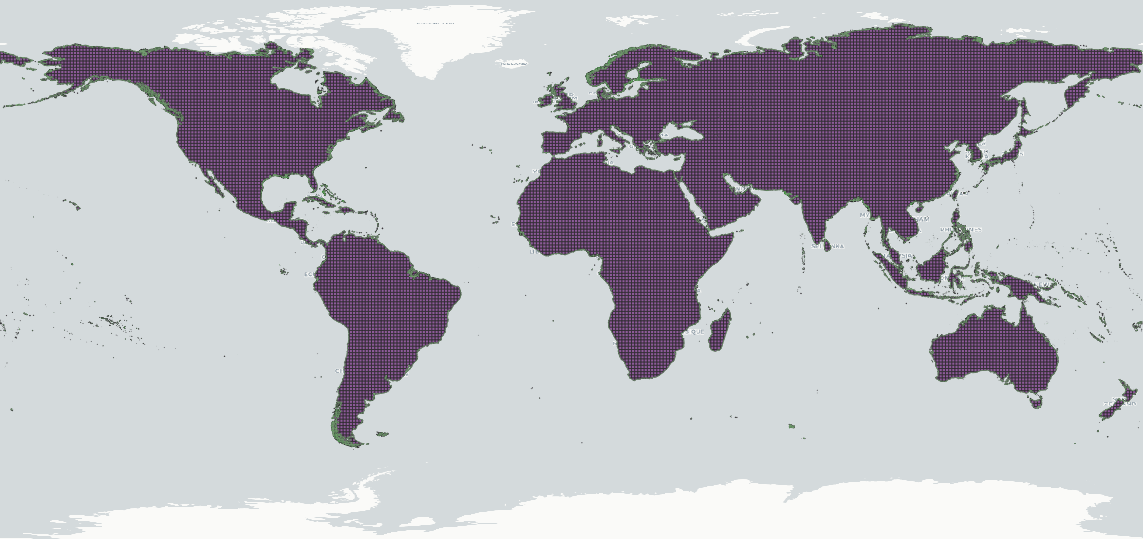
\includegraphics[width=\textwidth]{fig/part_2/S2Coast2023.png}
	\caption{-- Область суши и береговая линия выделенная в S2Coast-2023}
	\label{pic:S2Coast2023}
    \end{center}
\end{figure}

\subsubsection{Заключение}

На протяжении восьми столетий картографирование береговой линии прошло путь от визуального обобщения мореходного опыта в портуланах до автоматического извлечения субпиксельных контуров из мультиспектральных спутниковых снимков. 
Для современных исследовательских задач наиболее гибким инструментом является CoastSat на платформе GEE, OSM Coastlines (как наиболее актуальный и детальный набор глобальных векторных данных) и S2Coast-2023 как методологически согласованные глобальные данные. 
